%--------------------
% --- Title stuff ---
%--------------------

\newcommand{\mytitle}{BOEIend!} % chktex 8
\newcommand{\mysecondtitle}{Intermediate Report} % chktex 8
\newcommand{\footertitle}{BOEIend! -- Intermediate Report} % chktex 8
\newcommand{\mysubtitle}{Lab} % chktex 8
\newcommand{\mygroup}{Group 2} % chktex 8
\newcommand{\myauthor}{Birgen Vermang -- Sander Thierens -- Brecht Van Eeckhoudt\\ Louis Devreese -- Sarah Goossens} % chktex 8
\newcommand{\mycourse}{Mobile Communications} % chktex 8
\newcommand{\myclass}{MELICTETC \& MELICTICT} % chktex 8


% -----------------------------------
% --- Basic settings and packages ---
% -----------------------------------
\documentclass[11pt,a4paper,twoside]{article} %"twoside" for double sided printing
\usepackage[a4paper,margin=3cm,marginparwidth=2.5cm]{geometry}   % Paper size and margins

\usepackage[english]{babel}                 % Culturally-determined typographical rules
\usepackage[utf8x]{inputenc}                % Input accents characters from keyboard
\usepackage{amsmath}                        % Math stuff

\usepackage{graphicx}                       % Insertion of pictures
\usepackage{float}							% [H]
\usepackage{booktabs}						% Toprule, midrule, bottomrule
\usepackage{wasysym}			            % \Square command
\usepackage{marvosym}                       % \Male \Female $\EUR$
\usepackage{MnSymbol}                       % \diameter
\usepackage[electronic]{ifsym}			    % \RaisingEdge
\usepackage{soul}							% Highlight with \hl{}

\usepackage[colorinlistoftodos]{todonotes}  % Todo notes
\usepackage[T1]{fontenc}                    % All underscores use ttt font

\usepackage{hyperref}                       % Hyperlinks in table of contents and links
\def\UrlBreaks{\do\/ \do-} % chktex 21		% Let Hyperlinks break at / and -
\renewcommand\UrlFont{\color{blue}\ttfamily} % Change URL style and color to blue
\usepackage{url}							% Let URL's break at certain points

\usepackage[labelfont=bf]{caption}          % Caption labels in bold
\setlength{\parindent}{0em}                 % No new paragraph indentation
\setlength{\parskip}{1em}                   % Space between paragraphs

\usepackage[nottoc,notlot,notlof]{tocbibind} % Make references show up in table of contents
\usepackage{tocloft}                        % Add dots to all lines in table of contents
\renewcommand{\cftsecleader}{\cftdotfill{\cftdotsep}}

\usepackage{gensymb}                        % \degree


% -----------------------
% --- Custom commands ---
% -----------------------
% \link{https://...}
\DeclareRobustCommand{\link}[1]{{\underline{\textcolor{blue}{\texttt{#1}}}}} % Underline in blue

% \hl{} \hlcyan{}
\DeclareRobustCommand{\hlcyan}[1]{{\sethlcolor{cyan}\hl{#1}}} % Highlight in cyan


% -----------------------
% --- Header & Footer ---
% -----------------------
\usepackage{lastpage}                       % Last page reference
\usepackage{fancyhdr}                       % Fancy headers & footers
\pagestyle{fancy}                           % Enable fancy headers
\fancyhf{}                                  % Clear all headers and footers
\renewcommand{\headrulewidth}{1pt}          % Enable header line
\renewcommand{\footrulewidth}{1pt}          % Enable footer line
\fancyhead[C]{\mycourse{}: \mysubtitle{}: \mytitle} % Set new header center
\fancyfoot[LO,RE]{\footertitle} 
% Set new page numbering left even right oneven
\fancyfoot[LE,RO]{\thepage{} of~\pageref{LastPage}} 
% Redefine plain style, it is used for pages with new chapters
\fancypagestyle{plain}{
    \fancyhf{}
    \fancyfoot[LE,RO]{\thepage{} of~\pageref{LastPage}}
    \fancyfoot[LO,RE]{\footertitle} 
    \fancyhead[C]{\mycourse{}: \mysubtitle{}: \mytitle} 
    \renewcommand{\headrulewidth}{1pt}
    \renewcommand{\footrulewidth}{1pt}
}


% -----------------------------
% --- Other useful packages ---
% -----------------------------
\usepackage{minted}                         % Syntax highlighting
\setminted[vhdl]{linenos=true,frame=lines,fontsize=\footnotesize,framesep=2mm,tabsize=3,breaklines=true}

\usepackage{tcolorbox}  					% Colored boxes (methods, ...)
\tcbset{toptitle = 1mm, bottomtitle = 1mm, fonttitle = \bfseries} % Slightly more space above and below title, bold title

%\usepackage{chngcntr}						% Alternate figure and table numbering
%\counterwithin{figure}{section}			% Label figures by section
%\counterwithin{table}{section}				% Label tables by section

%\usepackage[none]{hyphenat}					% Disable all hyphenation in entire text



%----------------------------------------------------------------------------------------
%	BEGIN OF DOCUMENT
%----------------------------------------------------------------------------------------

\begin{document}

%----------------------------------------------------------------------------------------
%	TITLE PAGE
%----------------------------------------------------------------------------------------

\begin{titlepage}																			
	\newcommand{\HRule}{\rule{\linewidth}{0.5mm}} % Change thickness of lines																																		
	\center{} % Center everything on the page

	
\includegraphics[scale=0.55]{logo_kuleuven.png}\\
	\textsc{\large faculty of engineering technology\\-- gent --}\\[2cm]

	\textsc{\LARGE \MakeUppercase{\mycourse}}\\[0.25cm] % Major heading - course name
	\textsc{\Large \MakeLowercase{\mysubtitle}}\\[0.25cm] % Minor heading - course title

	\HRule \\[0.7cm] % chktex 1
	{ \huge \bfseries \mytitle \\[0.4cm] \MakeUppercase{\mysecondtitle}} \\[0.4cm] % Title of your document
	\HRule \\[1.4cm] % chktex 1
	
	{ \Large \MakeUppercase \mygroup } \\[0.4cm]
	
	\Large \myauthor \\[0.4cm] % chktex 1
	\large \myclass
	\\[1.4cm]

	{\Large \today }\\[1.4cm] % Date, change the \today to a set date if you want to be precise

	%\todo[inline, color=green!40]{Scalen pagina bij afdrukken uitzetten}

	%\vfill % Fill the rest of the page with whitespace

\end{titlepage}



%----------------------------------------------------------------------------------------
%	TABLE OF CONTENTS & ABSTRACT
%----------------------------------------------------------------------------------------

\tableofcontents
\vspace{1cm}

%\begin{abstract}\todo{Aanvullen!}
%Hier kan info voor een `abstract' komen. We typen redelijk veel tekst voor te laten zien waarin de tekst zich standaard in uitlijnt.

%We zien dat ook standaard een nieuwe paragraaf wordt aangeduid op de `Amerikaanse' methode.
%\end{abstract}

%\clearpage

%----------------------------------------------------------------------------------------

%\section*{Info}

%{ \footnotesize

%\hl{This is here just for reference and won't be submitted in the final document.}


%\begin{tcolorbox}[colback=red!5!white,colframe=red!75!black,title=Source material]
%	[1] Barbara J Hoogenboom and Robert C Manske. How to write a scientific article. International journal of sports physical therapy, 7(5):512, 2012.\\

%    [2] Elena D Kallestinova. How to write your first research paper. The Yale journal of biology and medicine, 84(3):181, 2011.
%\end{tcolorbox}

%\begin{tcolorbox}[colback=red!5!white,colframe=red!75!black,title=Intermediate Report -- 22/10/2018]
%	After the first session, each group must submit a report. This report must demonstrate that you have examined the use case and are capable of designing a viable solution. This includes a plan for a specification of the interfaces, selection of communication technologies (and why). The report needs to be submitted via e-mail to \texttt{gilles.callebaut@kuleuven.be} (before 22h00 at the day of the deadline).

%    \begin{description}
%        \item [File name format] \texttt{mobile\_comm\_group<nr>\_intermediate\_report.pdf}
%        \item [Language] Dutch or English (recommended)
%        \item [Number of pages] Write your report in a compact but concise way, following the strategies presented in [1, 2]. The report is also expected to be structured and styled as described there. The structure of the report will be taken into account when grading the report. This also holds for the final report.
%    \end{description}
%\end{tcolorbox}

%\begin{tcolorbox}[colback=orange!5!white,colframe=orange!75!black,title=Points to be discussed]
%	\begin{itemize}
%	    \itemsep0em
%	    \item Understand the problem statement
%	    \item Break the problem in smaller sub-problems
%	    \item Define the requirements for each problem
%	    \begin{itemize}
%	        \itemsep0em
%	        \item Parameterize each problem as much as possible (most often there are some assumptions you need to make)
%	        \item Select the wireless technologies based on the defined requirements
%	        \item Design strategies to detect drifting
%	        \item Utilize approaches to lower the overall energy consumption. You may also include recommendation for hardware related energy improvements.
%	    \end{itemize}
%	    \item Which problems could occur and how do you plan to tackle them?
%	    \item An economical point-of-view of the project needs to considered, i.e. what is the cost and the gain? Are there legal limitations?
%	    \item What are the technical limitation of the designed system?
%	    \item How to take energy efficiency and robustness into account?
%	\end{itemize}
%\end{tcolorbox}
%
%}

%\clearpage

%----------------------------------------------------------------------------------------
%	>>>>> START DOCUMENT <<<<<
%----------------------------------------------------------------------------------------

\section{Description of the problem}

\textit{`BOEIend!'} is a project about giving buoys the ability to communicate with each other, to make them `smart', so they can \textbf{automatically detect and report if they are adrift}. They can also periodically report other useful data such as \textbf{wave amplitude and water temperature}.

The goal of the project (and the lab sessions) is to \textbf{develop the design and specifications for the communication element of such a `smart' buoy}, and to \textbf{build and test a prototype}. Buoys generally have a lifespan of \textbf{5-10 years} so the design must be \textbf{energy efficient} and possibly make use of some energy-harvesting methods.

Since the scope of the lab is more about the communication-side, the low-power aspect should rather be kept in mind than to actively pursued. We know however that due to the limited energy budget of some of the buoys, continuous collecting GPS measurements is unfeasible. It is thereby imperative that low-energy strategies are employed to ensure a long lifespan. We can also see that we need to look more into other localization or proximity-based mechanisms.

\clearpage

%----------------------------------------------------------------------------------------

\section{Breakdown in smaller sub-problems}

\subsection{Types of buoys}

We can divide our problem in smaller sub-problems by distinguishing two types of buoys:

\begin{description}
    \item [Master buoy] These buoys will be equipped with the technology required to communicate with both the mainland and the other (slave) buoys. It is important to use a technology that is capable of communicating over rather long distances for the connection to the mainland. 
    
    These larger buoys will be equipped with larger batteries. For the scope of this coarse we can assume they have `unlimited power', so they can be used to do more energy-heavy tasks.
    
    \item [Slave buoy] These buoys need to be energy-efficient and could generate their own energy. They don't need to communicate over long distances.
\end{description}

On figure~\ref{fig:problem} we see a diagram of the general problem. In this project, we assume the following distances:
\vspace{-0.4cm}
\begin{itemize}
    \itemsep0em
    \item Coast $\leftrightarrow$ Master buoy (A): 100 m -- 1 km
    \item Neighboring (slave) buoys (B): 10 m
    \item Immobile buoy $\leftrightarrow$ drifting buoy (C): > 20 m
\end{itemize}

A buoy is considered \textbf{out of place} when the distance to his original location is lager than a certain predefined threshold, which is in this case \textbf{20 meters}.

\begin{figure}[H]
    \begin{center}
        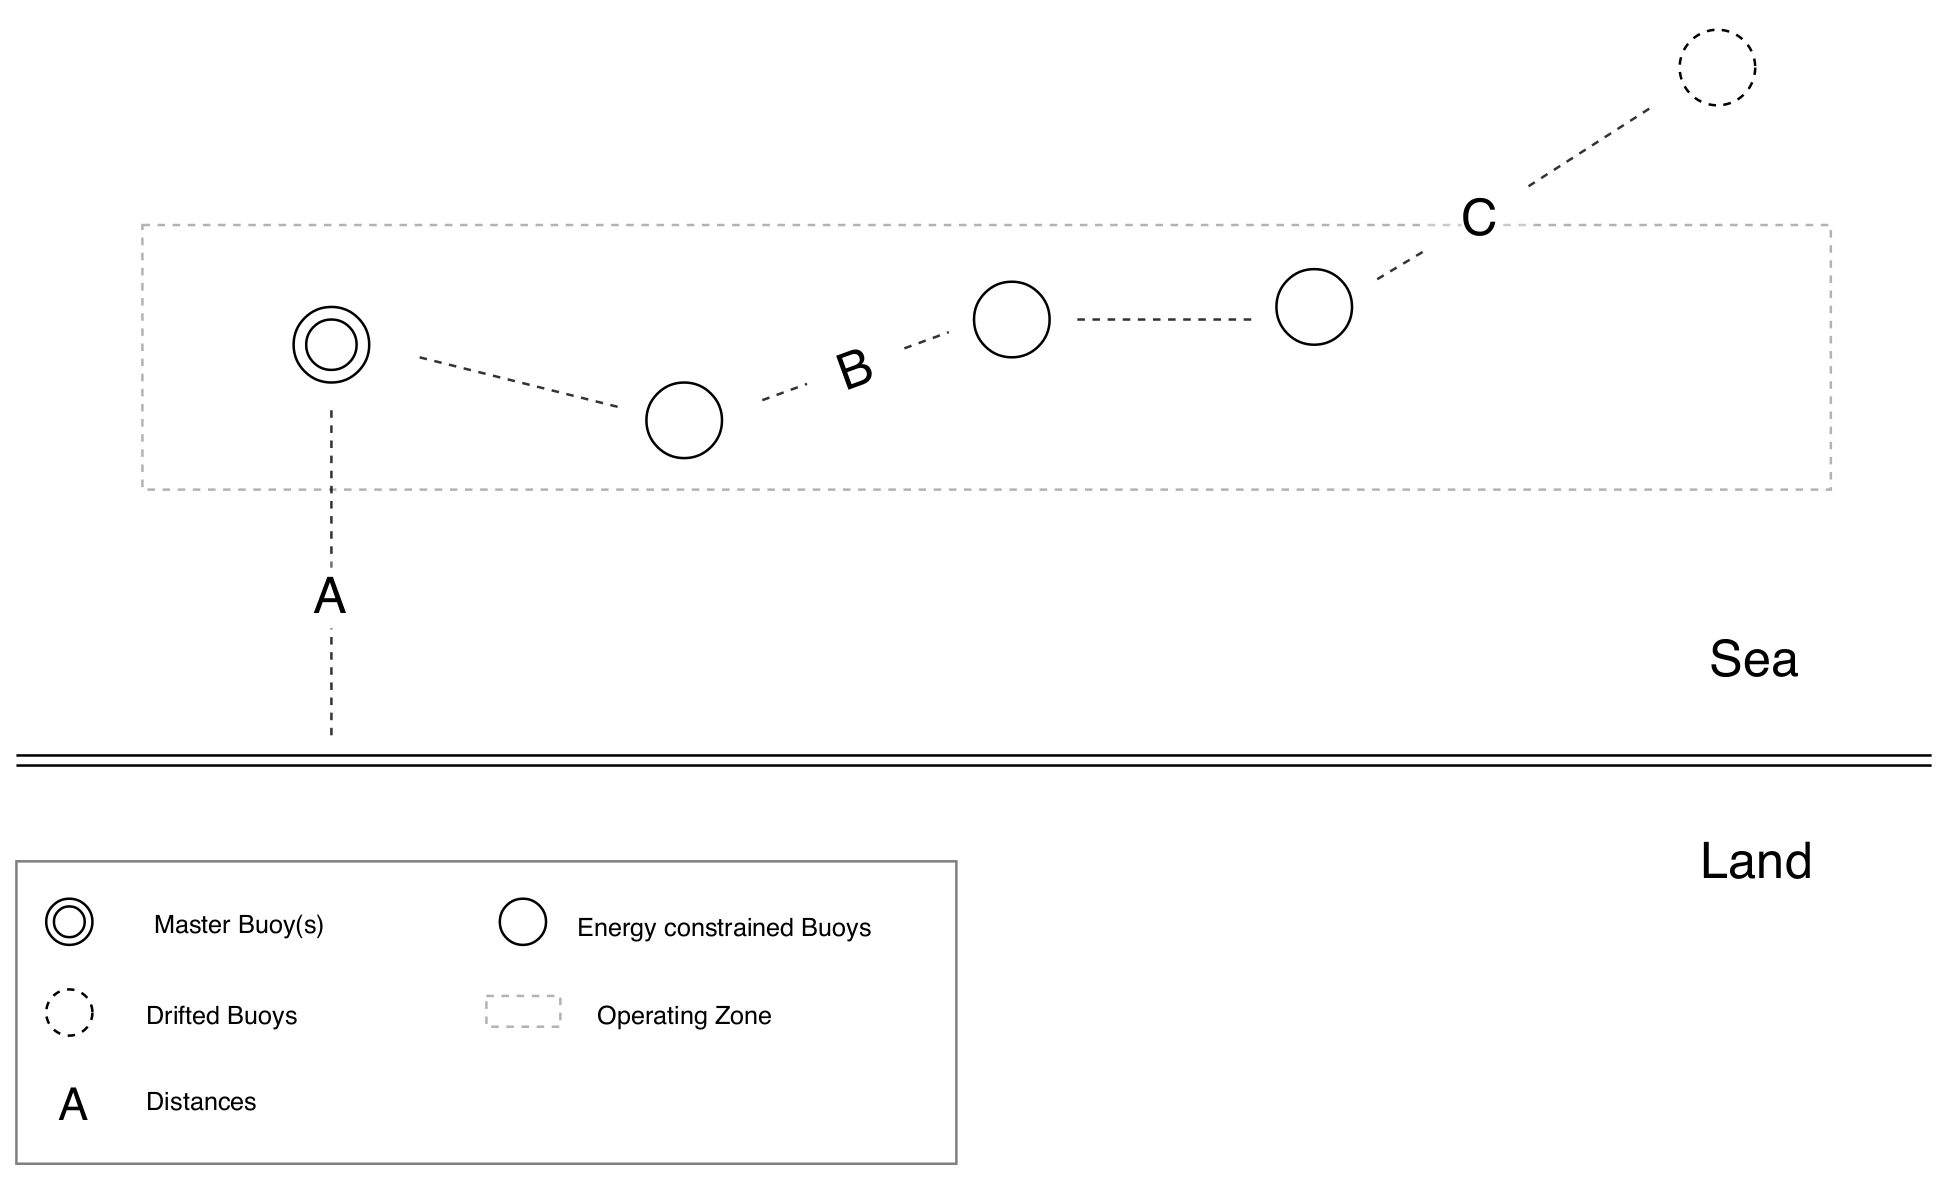
\includegraphics[width=1.0\textwidth]{problem.png}
        \caption{\label{fig:problem}Visualization of the project.}
    \end{center}
\end{figure}

\clearpage



\subsection{Communication to the mainland}

Communication \textbf{between the mainland and the `master' buoys} will be established using a \textbf{LoRa-connection}. Reasons to choose for LoRa in our case include the great range and the low power-consumption. On the master buoys we theoretically have an `unlimited' amount of power, but a low power design is always preferred.

The LoRaWAN network by Proximus~\cite{LORAWAN} covers almost the whole area of Belgium, as depicted on Figure~\ref{fig:Coverage}. We can see that the network reaches a few kilometers in to the North Sea. This makes it a perfect candidate for our connection between the master buoys (equipped with a LoRa-module) and the mainland. The data coming from the master buoys will be transmitted over the LoRa network to `the cloud', where it can be collected and further analyzed.

In the lab sessions we will experiment with a \fbox{\texttt{EMF32 Happy Gecko} development-board} with a \fbox{\texttt{DRAMCO LoRaWAN RN2483} modem addon board}.

\begin{figure}[H]
    \centering
    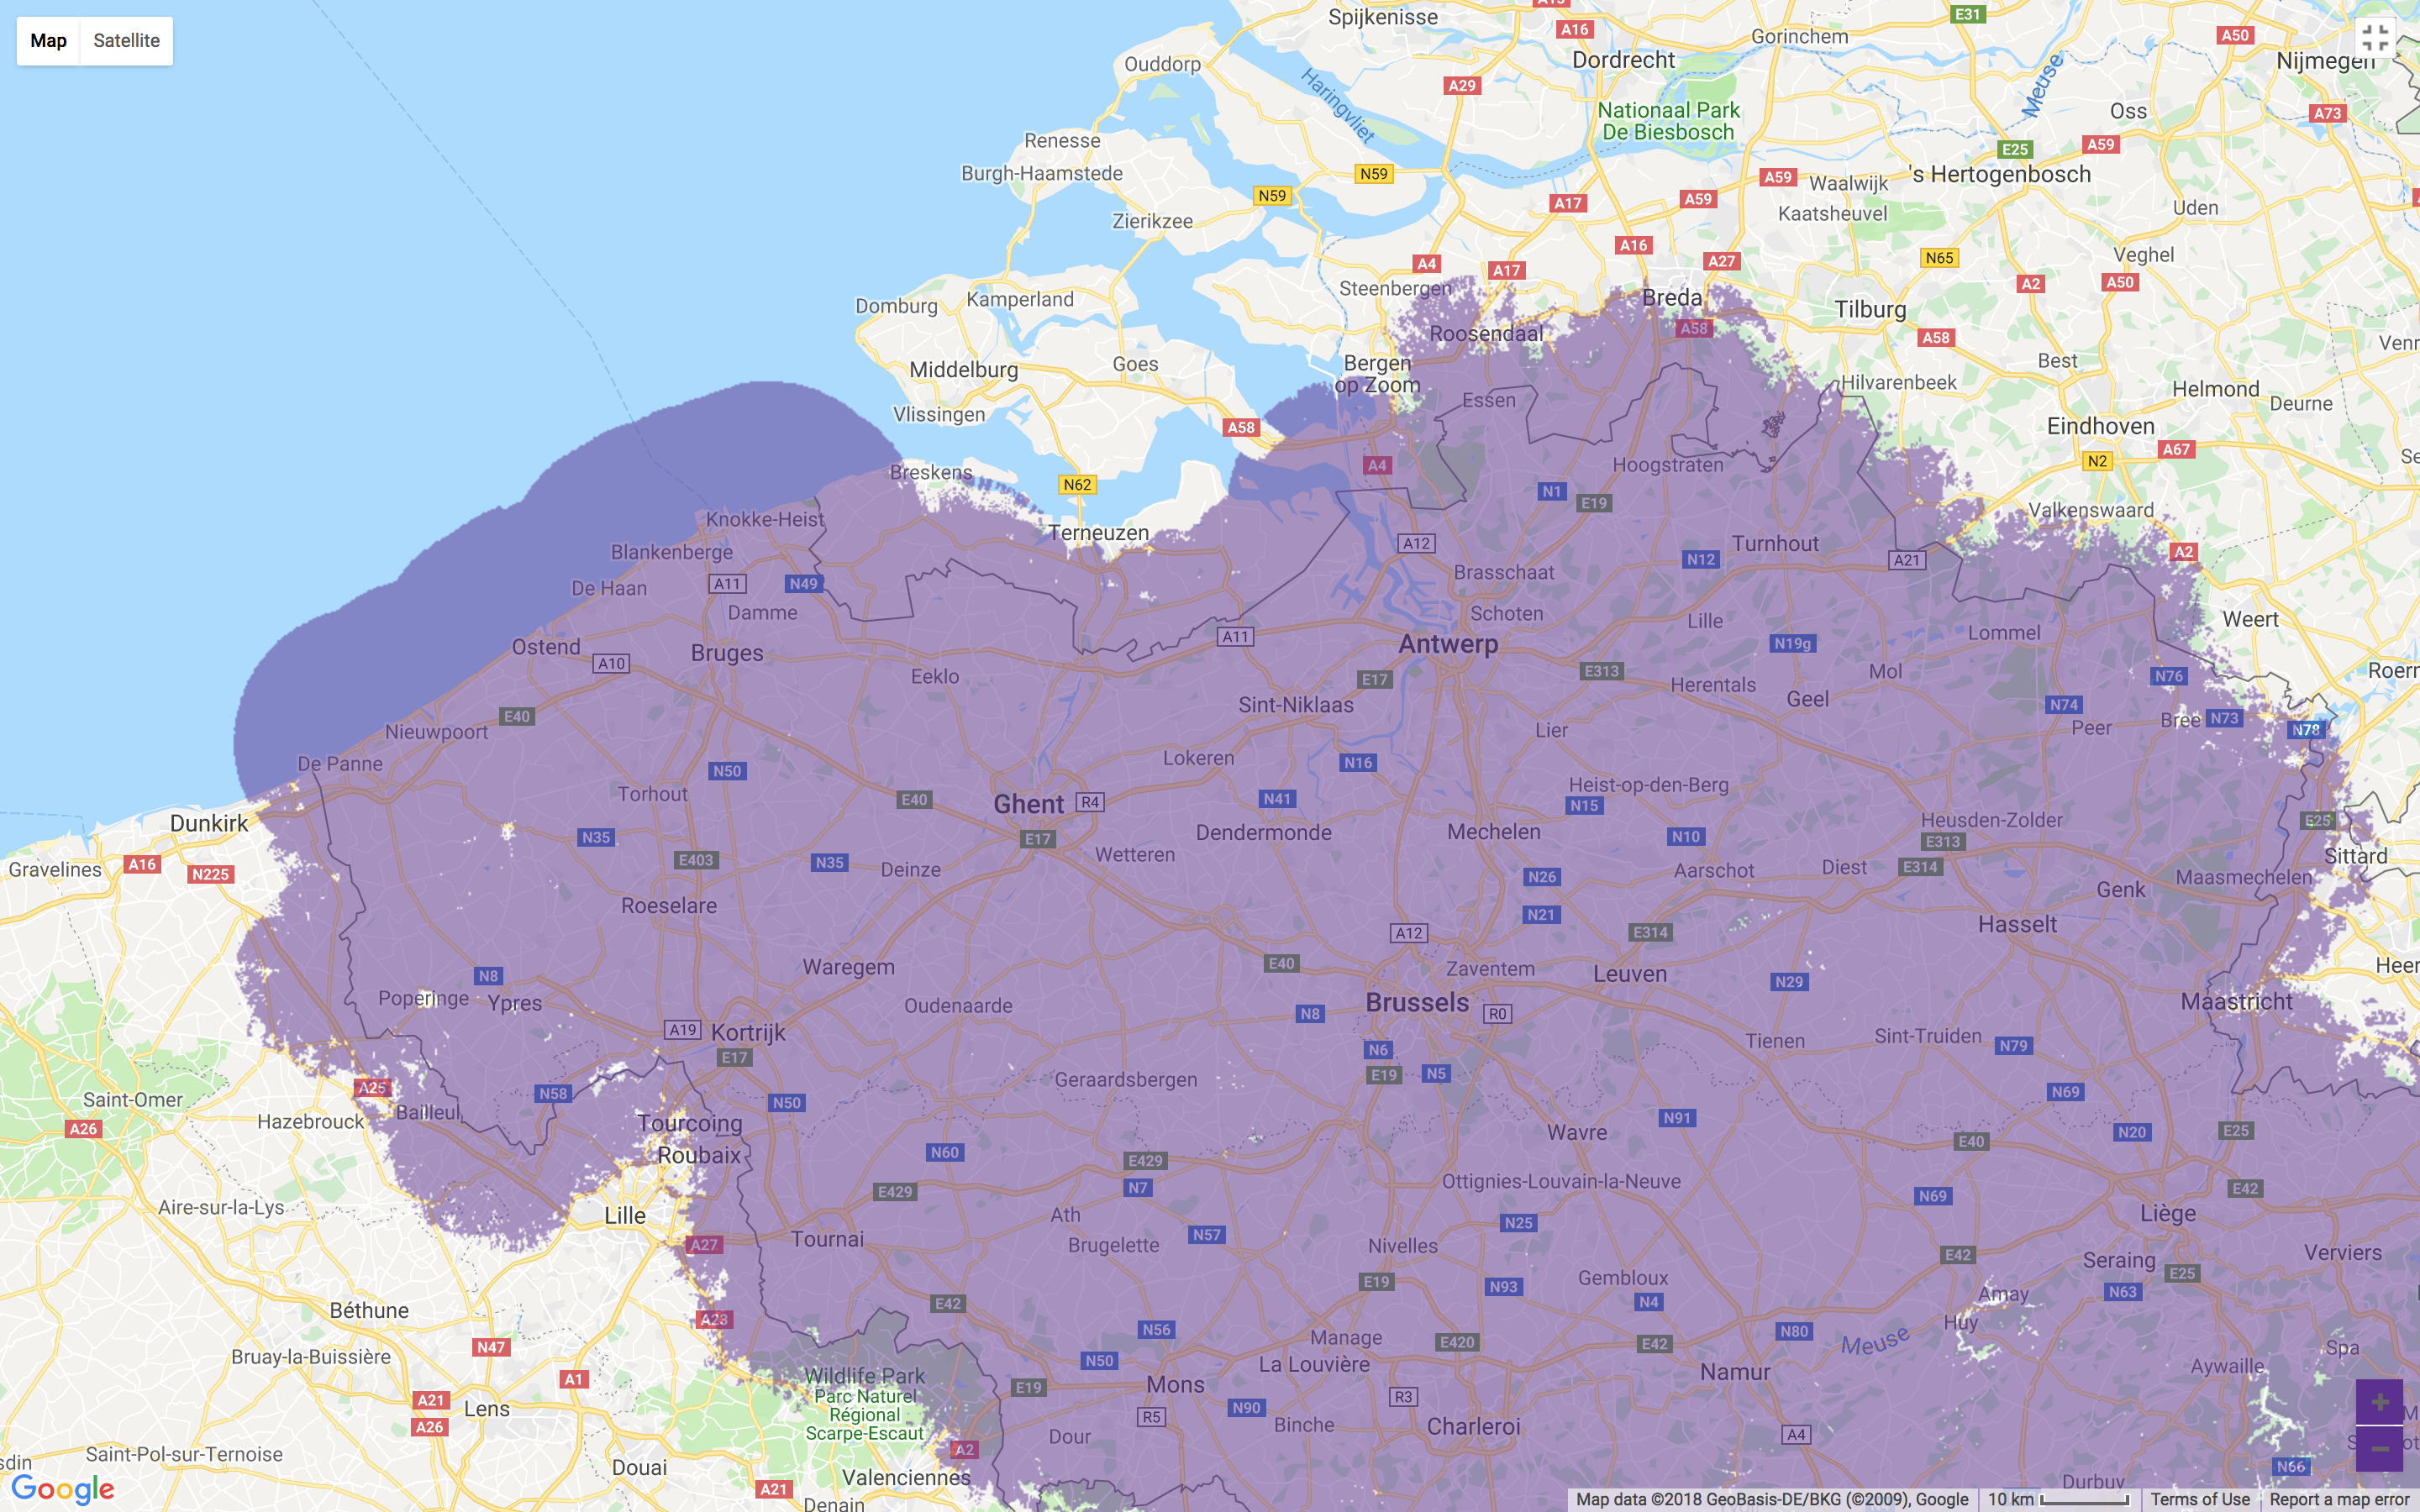
\includegraphics[width=0.8\textwidth]{LoraDekking.png}
    \caption{Coverage of the LoRaWAN-network by Proximus.}
    \label{fig:Coverage}
\end{figure}

\clearpage


\subsection{Communication between buoys}

Starting with the data given in our assignment (also depicted on figure~\ref{fig:problem}) we can see that each buoy and the next will be \textbf{10 meters} apart. If we determine that \textbf{every 15 buoys a master buoy} is needed, we can see that the master buoy needs a communication protocol which is able to communicate in a \textbf{star-network of up to 70 meters}. This means that every master buoy needs to communicate with 7 buoys to the left and 7 buoys the right. An overview of this proposed implementation is shown in Figure~\ref{fig:Overview}.

A communication technology that can handle these distances is \texttt{Zigbee}. With this technology every `slave' buoy will communicate with the master in a star topology. When all the buoys are in the right position and the distance between every master buoy is 150 meters, each slave buoy within a distance of maximum 70 meters (if he is at his correct position) can communicate with his designated master buoy. This also means that \textbf{a drifting buoy} can communicate with the master buoy \textbf{if it stays at a distance of maximum 100 meters}, which corresponds to \textbf{30 meters drifting}.

To realize this we will be using a \fbox{\texttt{DRAMCO ZigBee} Arduino Shield}.

\begin{figure}[H]
    \centering
    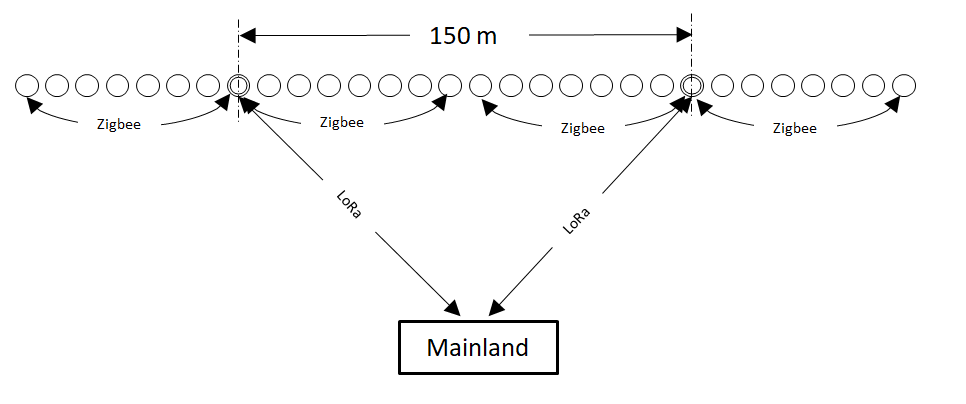
\includegraphics[width=1.0\textwidth]{opstelling.png}
    \caption{The overview of the proposed implementation.}
    \label{fig:Overview}
\end{figure}

\clearpage

%----------------------------------------------------------------------------------------

\section{Technologies}

\subsection{LoRa}

LoRa is a communication technology developed by SEMTECH. By using sub-Gigahertz radio band frequencies, this technology has a very wide range with limited power consumption. Because they work on lower frequencies the error-bit rate is significantly lower, but this will also result in a lower data-bit rate. All of these features make LoRa a suitable communication protocol for the connection between the master buoys and the mainland.

\subsection{ZigBee}

ZigBee is an IEEE 802.15.4-based specification for a suite of high-level communication protocols used to create personal area networks with small, low-power digital radios. Use-cases can be found in home automation, medical device data collection and other low-power low-bandwidth needs. This communication technology can communicate between 10 and 100 meters with a bit rate of approximately 0,12 Mbit/s.\cite{Zigbee}

%----------------------------------------------------------------------------------------
%	BIBLIOGRAPHY
%----------------------------------------------------------------------------------------

%\clearpage
\vspace{1.5cm}
			
\begin{thebibliography}{9}
    \bibitem{LORAWAN} Proximus, \textit{LORAWAN},\\
	\url{https://www.proximus.be/en/id_cl_iot/companies-and-public-sector/solutions/connected-business/internet-of-things.html}
	\bibitem{Zigbee} Wikipedia, \textit{ZIGBEE},\\
	\url{https://en.wikipedia.org/wiki/Zigbee}
\end{thebibliography}

	

\end{document}